\documentclass[
    a4paper,            % Paper size
    11pt,               % Font size
    stu,                % Format as assignment
    donotrepeattitle,   % Start body text without repeating title
    noextraspace,       % Reduce spaces between section header and text
    floatsintext,       % Insert tables and figures with texts
    biblatex,           % Use BibLaTeX for references
    colorlinks=true,        % Colour all links
    linkcolor=red,          % Cross-references in red
    anchorcolor=black,      % Keep anchors black
    citecolor=blue,         % In-text-referencs in blue
    urlcolor=blue,          % DOIs and URLs are in blue
    bookmarks=true,         % Generate bookmarks for PDF readers
    bookmarksopen=false,    % Expand all bookmarks as default
    bookmarksnumbered=true  % Keep section number in bookmarks
]{apa7}

% Avoid breaking a word into two lines
\usepackage[none]{hyphenat}

% Activate AMS packages for typing maths
\usepackage{amsmath,amssymb}

\newcommand{\p}[1]{\mathbb{P}\left(#1\right)}
\newcommand{\E}[1]{\mathbb{E}\left(#1\right)}
\renewcommand{\exp}[1]{\mathrm{exp}\left\{#1\right\}}

% Insert images
\usepackage{graphicx}

% Change line spacing
\usepackage{setspace}
\setstretch{2}

\usepackage[nameinlink,noabbrev,capitalise]{cleveref}

% Package biblatex has already been loaded by apa7.
% Only need to specify the bib library
\addbibresource{../../Bibliography/Master.bib}
\newcommand{\poscite}[1]{\citeauthor{#1}'s (\citeyear{#1})}

\title{A quantitative enquiry into the fairness and equity in Norwegian secondary school assessment practices: Project proposal}
\author{Tony C. A. Tan}
\affiliation{Centre for Educational Measurement, University of Oslo}
\course{UV9040A Research Seminar}
\professor{Associate Prof Bj{\"o}rn Andersson}
\duedate{14 September 2021}

\begin{document}
\maketitle

\section{Introduction}

%//mark State the research problem
%//tip Write an opening sentence that will stimulate reader interest as well as convey an issue to which a broad audience can relate.
%//tip As a general rule, refrain from using quotations--especially long ones--in the lead sentence because it will be difficult for readers to grasp the key idea you would like for them to see. Quotations raise many possibilities for interpretation and thus create unclear beginning. However, as is evident in some qualitative studies, quotations can create reader interest.
%//tip Stay away from idiomatic expressions or trite phrases (e.g., "The lecture method remains a 'sacred cow' among most college and university instructors.").
%//tip Consider numeric information for impact (e.g., "Every year, an estimated 5 million Americans experience the death of an immediate family member.").
%//tip Clearly identify the research problem (i.e., dilemma, issue) leading to the study. Ask yourself, "Is there a specific sentence (or sentences) in which I convey the research problem?"
%//tip Indicate why the problem is important by citing numerous references that justify the need to study the problem. In perhaps a lesson than joking manner, we say to our students that if they do not have a dozen references cited on the first page of their proposal, they do not have a scholarly study.
%//tip Make sure that the problem is framed in a manner consistent with the approach to research in the study (e.g., exploratory in qualitative, examining relationships or predictors in quantitative, and either approach in mixed methods inquiry).
%//tip Consider and write about whether there is a single problem involved in the proposed study or multiple problems that lead to a need for the study. Often, multiple research problems are addressed in research studies.

Based on \textit{Statistisk sentralbyr{\aa}} archive \parencite{ssb:completion}, 34,660 young Norwegians between 2014 and 2020 entrusted their future to the grade point average (GPA) system upon completion of their secondary schools (general studies). Although the public \emph{assumes} axiomatically the GPA-based selection system to be fair, little theoretical and empirical efforts had been devoted to the detailed examination of such claim in the Norwegian context. The fairness of this trust-based selection system is further called into question by the increasing dissenting voices overseas. By analysing UK's 2004 General Certificate of Secondary Education data, for instance, \textcite{coe:2008} revealed significant differences in subject difficulties, with some being more than one grade harder than others. Similarly in the Netherlands, \textcite{korobko:2008} reported comparable heterogeneity in subject difficulties using the Central Examinations in Secondary Education data. Cross country comparisons by \textcite{lamprianou:2009} also revealed significant differences in assessment practices for the purpose of enhancing test fairness. When test difficulties vary across subjects, winners and losers are created; delays in re-aligning subject difficulties during GPA calculations would erode public trust in the impartiality, therefore the legitimacy, of university entry selection process.

%//mark Review studies that have addressed the problem
%//tip Refer to the literature by summarising groups of studies, not individual ones. The intent should be to establish broad areas of research.
%//tip To de-emphasise single studies, place the in-tex references at the end of a paragraph or at the end of a summary point about several studies.
%//tip Review research studies that used quantitative, qualitative, or mixed methods approaches.
%//tip Find recent literature to summarise, such as that published int he past ten years. Cite older studies if they are valuable because they have been widely referenced by others.

Enquiries into subject difficulty re-calibration have a long history. \textcite{tognolini:1996} used extended logistic models to measure the latent trait of test candidates. In addition to their detailed mathematical derivations, theses authors made extensive justification for the viability of summarising learners' diverse capabilities into a single score, paving the way for subsequent research efforts using Rasch modelling. Parallel to empirical studies, advancement in estimation methods also enabled the proliferation of Rasch modellings. Three main approaches to parameter estimation have withstood the test of time: marginal maximum likelihood estimation \parencite[MML, ][]{bock:1981} where person parameters are treated as random effects and are integrated out of the likelihood function, joint maximum likelihood estimation \parencite[JML, ][]{birnbaum:1968, lord:1980, mislevy:1987} where person parameters are treated as fixed effects and are retained in the likelihood function, and conditional maximum likelihood estimation \parencite[CML, ][]{andersen:1972}, which takes advantage of the separability of the person and subject parameters in a Rasch model to condition the likelihood function on its sufficient statistics. Recent studies suggested CML over its competitors thanks to its computational efficiency \parencite{christensen:2013} and robustness to normality violation \parencite{steinfeld:2021}.

%//mark Indicate deficiencies in the studies
%//tip Cite several deficiencies to make the case even stronger for a study.
%//tip Identify specifically the deficiencies of other studies (e.g., methodological flaws, variables overlooked).
%//tip Write about areas overlooked by past studies, including topics, special statistical treatments, significant implications, and so forth.
%//tip Discuss how a proposed study will remedy these deficiencies and provide a unique contribution to the scholarly literature.

%//mark Advance the significance of the study for particular audiences
%//tip Three or four reasons that the study adds to the scholarly research and literature in the field
%//tip Three or four reasons about how the study helps improve practice
%//tip Three or four reasons as to why the study will improve policy or decision making

The current study responses to the under-research in Norway's GPA architecture. It is particularly interested in knowing whether the GPA in its present form is a ``fair'' measure of candidates' underlying capabilities. More specifically, fairness is conceptualised as the comparability in difficulty levels across subjects such that no candidate shall be favoured or penalised for their subject choices. Should significant differences in subject difficulties be found, research interests would be devoted to the spatial-temporal distribution (Which subjects are the easiest/hardest? Do these differences occur only in one particular year or in every year? Are these differences getting bigger, smaller, stable or fluctuate over the years?), causes (Why?), personal impact (Who are mostly (dis-)advantaged by such differences?) as well as policy actions (What can be done to address such unfairness?). On the contrary, should this study find no significant difference, it would also serve Norway's interest well by lending support and legitimacy to its current university entry selection mechanism. Results from this project directly benefit students and their parents through enhanced transparency and accountability of a system that determines their future and dreams. Educators and decision makers may also derive utility from this study for their evidence-based policy design.

%\section{Purpose Statement}

%//mark establish the intent of the entire research study
%//mark needs to be clear, specific, and informative

%//tip The purpose statement sets the objectives, the intent, or the major idea of a proposal or a study. This idea builds on a need (the problem) and is refined into specific question (the research questions).

%//tip Include words to signal the major intent of the study, such as purpose, intent, or objective. Start with "The purpose (or objective or intent) of this study is (was, will be)..."
%//tip Identify the theory, model, or conceptual framework. At this point, one does not need to describe it in details. Mentioning it in the purpose statement provides emphasis on the importance of the theory and foreshadows its use in the study.
%//tip Identify the independent and dependent variables, as well as any mediating or moderating variables used in the study.
%//tip Use words wht connect the independent and dependent variables to indicate that they are related, such as "the relationship between" two or more variables or a "comparison of" two or more groups. Also, a purpose statement could be to "describe" variables. Most quantitative studies employ one or more of these three options for discussing variables in the purpose statement. A combination of comparing and relating might also exist--for example, a two-factor experiment in which the researcher has two or more treatment groups as well as a continuous independent variable. Although one typically finds studies about comparing two or more groups in experiments, it is also possible to compare groups in a survey study.
%//tip Position or order the variables from left to right in the purpose statement--with the independent variable followed by the dependent variable. Place intervening variables between the independent and dependent variables. Many researchers also place the moderating variables as related to the independent variables. In experiments, the independent variable will always be the manipulated variable.
%//tip Mention the specific type of strategy of inquiry (such as survey or experimental research) used in the study. By incorporating this information, the researcher anticipates the methods discussion and enables a reader to associate the relationship of variables to the inquiry approach.
%//tip Make reference to the participants (or the unit of analysis) in the study, and mention the research site.
%//tip Generally define each key variable, preferably using set and accepted established definitions found in the literature. General definitions are included at this point to help the reader best understand the purpose statement. They do not replace specific, operational definitions found later when a writer has a "Definition of Terms" section in a proposal (detail about how variables will be measured). Also, delimitations that affect the scope of the study might be mentioned, such as the scope of the data collection or limited to certain individuals.

%\section{Research Questions}

%//tip The use of variables in research questions or hypotheses is typically limited to three basic approaches. The researcher may compare groups on an independent variable to see its impact on a dependent variable (this would be an experiment or group comparisons). Alternatively, the investigator may related one or more independent variables to one or more dependent variables (this would be a survey that correlates variables). Third, the researcher may descirbe responses to the independent, mediating, or dependent variables (this would be a descriptive study). Most quantitative research falls into one or more of these three categories.
%//tip The most rigorous form of quantitative research follows from a test of a theory and the specification of research questions or hypotheses that logically follow from the relationship among variables in the theory.
%//tip The independent and dependent variables must be measured separately and not measured on the same concept. This procedure reinforces the cause-and-effect logic of quantitative research.
%//tip To eliminate redundancy, write only research questions or hypotheses--not both--unless the hypotheses build on the research questions. Choose the form based on tradition, recommendations from an adviser or faculty committee, or whether past research indicates a prediction about outcomes.
%//tip If hypotheses are used, there are two forms: (a) null and (b) alternative. A null hypothesis represents the traditional approach: It makes a prediction that in the general population, no relationship or no significant difference exists between groups on a variable. The wording is, "There is no difference (or relationship)" between the groups.
%//tip The second form, popular in journal articles, is the alternative or directional hypothesis. The investigator makes a prediction about the expected outcome, basing this prediction on prior literature and studies on the topic that suggest a potential outcome. For example, the researcher may predict that "scores will be higher for Group A than for Group B" on the dependent variable or that "Group A will change more than Group B" on the outcome. These dxamples illustrate a directional hypothesis because an expected prediction (e.e.g, higher, more change) is made.
%//tip Another type of alternative statement is the non-directional hypothesis--a prediction is made, but the exact form of differences (e.g., higher, lower, more, less) is not specified because the researcher does not know what can be predicted from past literature. Thus, the investigator might write, "There is a difference" between the two groups.

With the aforementioned motivations, this study wishes to directly address the following research questions:
\begin{enumerate}
    \item[RQ1] To what extent can a Rasch model approximate Norway's GPA scores?
    \item[RQ2] Does the difficulty parameter differ significantly across subject?
    \item[RQ3] If the answer to RQ2 is ``yes'', then further RQs would involve:
        \begin{enumerate}
            \item[RQ3.1] Which are the easiest and hardest subjects?
            \item[RQ3.2] Are there any systematic differences by socio-demographic variables such as sex, immigration history or socio-economic spectrum?
            \item[RQ3.3] Do such differences remain stable over time?
        \end{enumerate}
\end{enumerate}

\section{Methods}

\subsection{Sample}

For this study, students' GPA records will be extracted from the Norwegian registry covering the period between 2006 (the year of education reform) and 2020 (most recent year with available data). GDPR registration is lodged through the NSD Portal and the UiO ethics approval is also obtained. All data import, storage, and analyses are to be conducted within the secured infrastructure TSD provided by the UiO Central IT Division. TSD logs all activities and no data or results can be copied out of the restricted system without prior approval from project leaders.

Under the advisory of \textcite{he:2015}, subjects with fewer than 1,000 candidates and students taking fewer than two GPA subjects will be excluded from subsequent analyses. Each year's record (score matrix) will contain $N$ rows representing the number of valid candidates and $L$ columns reflecting the usable number of GPA subjects in that year. Since no student took all the GPA subjects, a large proportion of the score matrices will remain missing by design. The existence of missing data does not pose any problems for using the Rasch model as the model functions at the individual subject and as long as there is sufficient overlap across subjects in the score matrix. The ability to deal with incomplete data is one major advantage of using the Rasch model for studying inter-subject comparability.

\subsection{Rasch Model}

The Rasch model was developed in the 1960s for establishing measurement scales and for improving test development \parencite{rasch:1980}. In a simple Rasch model, the underlying ability or latent trait of the person ($\theta$) and the item characteristics ($\delta_j$) are specified; a logistic function ($\Lambda$) is then used to describe the probability that the person will successfully pass a subject ($x_j=1$) given their ability $\theta$ and the item characteristics $\delta_j$ \parencite{deayala:2009}:
\begin{equation}\label{eq:di}
    \p{x_j = 1 | \theta, \delta_j} = \Lambda(\theta - \delta_j) = \frac{1}{1 + e^{- \left( \theta - \delta_j \right) } }.
\end{equation}

% Partial Credit Model
\cref{eq:di} is suitable for modelling subjects with dichotomous (pass/fail) outcomes. GPAs on the other hand are polytomous in nature (\S 3-5, \textit{Forskrift til oppl{\ae}ringslova}), therefore requires models capable of accommodating more than two achievement outcomes. Multiple extensions have been put forward over the decades such as rating scale models \parencite{rasch:1980}, partial credit models \parencite{masters:1982}, and generalised partial credit models \parencite{muraki:1992}. Master's (1982) partial credit models (PCM) are particularly parsimonious and flexible for studying the structure of GPA data. A PCM states that, for a subject with $m+1$ available grades ($m=5$ for Norway's GPA system), the probability of a candidate with ability $\theta$ receiving grade $x$ can be expressed as:
\begin{equation}\label{eq:pcm}
    \p{\theta, x}=
    \left\{
        \begin{aligned}
            &\frac{1}{1 + \sum_{l=1}^m \exp{ \sum_{k=1}^l (\theta - \delta_k) }}\ \ \ \text{for } x_j = 0\\
            &\frac{ \exp{ \sum_{k=1}^x (\theta - \delta_k) } }{1 + \sum_{l=1}^m \exp{ \sum_{k=1}^l (\theta - \delta_k) }}\ \ \ \text{for } x_j = 1,2,\dots,m
        \end{aligned}
    \right.
\end{equation}
where $\delta_k$ is the location of the $k$-th step on the latent trait continuum, often referred to as the item step parameter associated with a grade category, step difficulty or threshold. $\p{\theta, x}$ is commonly known as the category response function or the item category probability curve (CPC). Model parameters in \cref{eq:pcm} can be solved using conditional maximum likelihood estimation \parencite{andersen:1972}.

\subsection{Difficulty Parameters}

It is important to highlight that $\delta_k$ cannot be interpreted as the difficulty of scoring $k$ in a subject. \textcite{wu:2007} proposed measures of subject difficulty based on expected scores by first defining the item characteristic curve (ICC):
    $ \E{\theta} = \sum_{x=0}^m x\p{\theta,x}, $
then the difficulty of scoring $k$ ($d_k$) as the ability at which the expected score on the ICC is $k-0.5$:
\begin{equation}
    d_k = \theta | _{\E{\theta} = k - 0.5}.
\end{equation}
The overall difficulty of a subject ($D$) can be obtained by averaging all step parameters:
\begin{equation}
    D = \frac{1}{m} \sum_{k=1}^m \delta_k.
\end{equation}
This study aims to ascertain the grade difficulties ($d_k$) as well as the overall difficulty of each subject, similar to Figure 13 of \textcite{he:2015}:
\begin{figure}[ht]
    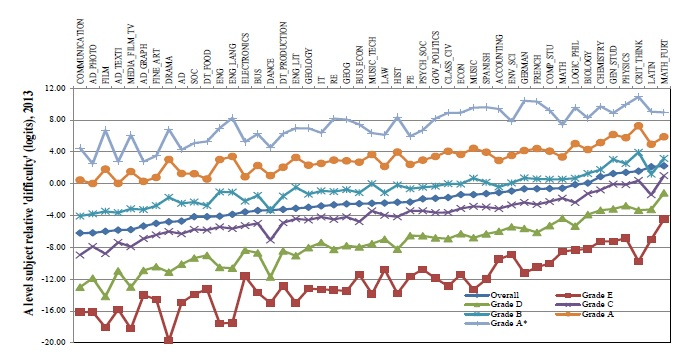
\includegraphics[scale=1]{expected_result.jpg}
    \centering
\end{figure}

\subsection{Data Analyses}

This study will make extensive use of STATA 17's IRT module. Based on recommendations from recent simulation studies \parencite{christensen:2013, steinfeld:2021}, CML will be used as the primary estimation procedure. Missing data require no additional treatment since one major advantage of IRT is its ability to handle dataset containing ``planned missingness''. Analyses will be repeated for each year, with the results forming a pooled cross sectional data for temporal comparisons (subject $\times$ grade $\times$ time).

%\subsection{Hypothesised Results}

\printbibliography

\end{document}